\vspace*{4cm}
\part{Bluetooth Mesh}\label{part:BluetoothMesh}
Raffael Anklin
\vspace*{\fill}
\clearpage

\section{Einleitung}\label{sec:EinleitungBluetooth}


Bluetooth Mesh ist ein auf dem Bluetooth-Standard aufbauendes Mesh-Netzwerk. Der Standard wurde im Jahr 2017 von der Bluetooth-SIG vorgestellt. Das Ziel des Standards ist es die Reichweite und das Einsatzgebiet von Bluetooth-Geräten zu erweitern. Somit sollen in Zukunft Lichtschalter und Lampen, sowie Sensoren und Aktoren im Heimbereich, Industriebereich und diversen Anwendungsbereichen mittels Bluetooth-Mesh verbunden werden.  \\

\begin{figure}[!htbp]
	\begin{minipage}{0.49\textwidth}
		\centering
		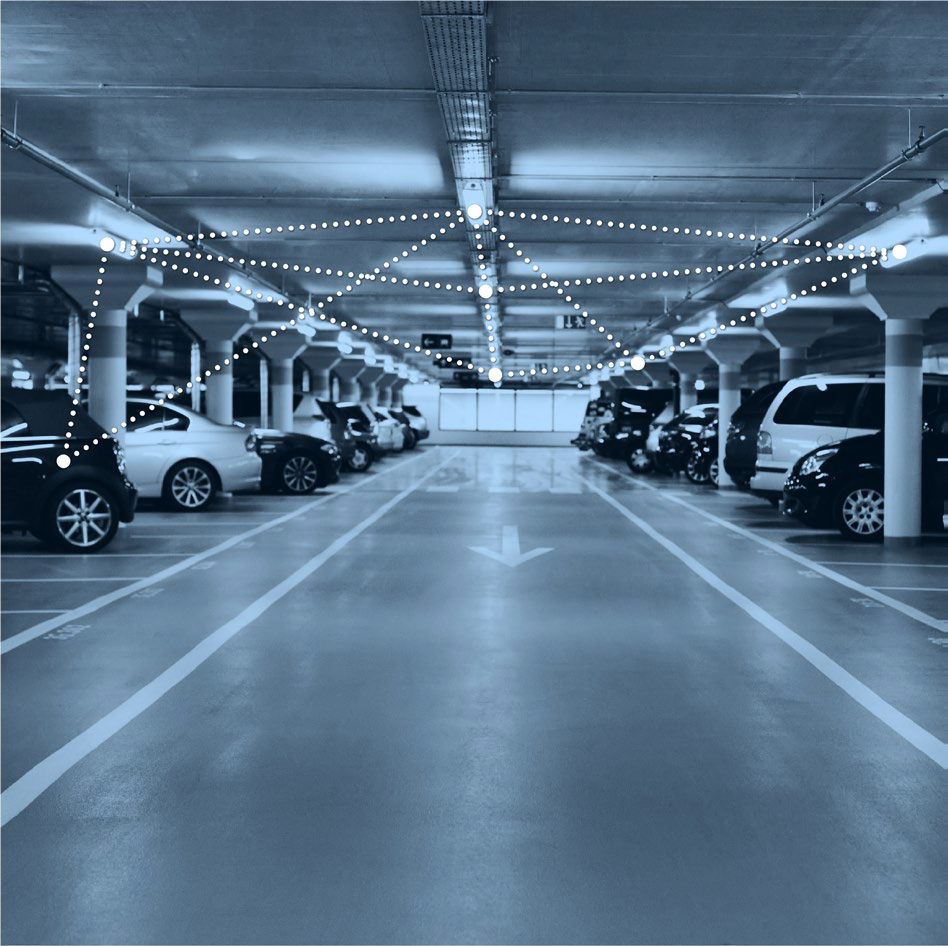
\includegraphics[width=\textwidth]{Bluetooth_Mesh_CarPark_Example.png}
		\caption[Beispielanwendung ]{CCA Prüfung (Idle Event) \cite{bluetooth_sig_mesh-technology-overviewpdf_2020}}
		\label{fig:BluetoothMeshParkingExample}
	\end{minipage}
	\begin{minipage}{0.49\textwidth}
		\centering
		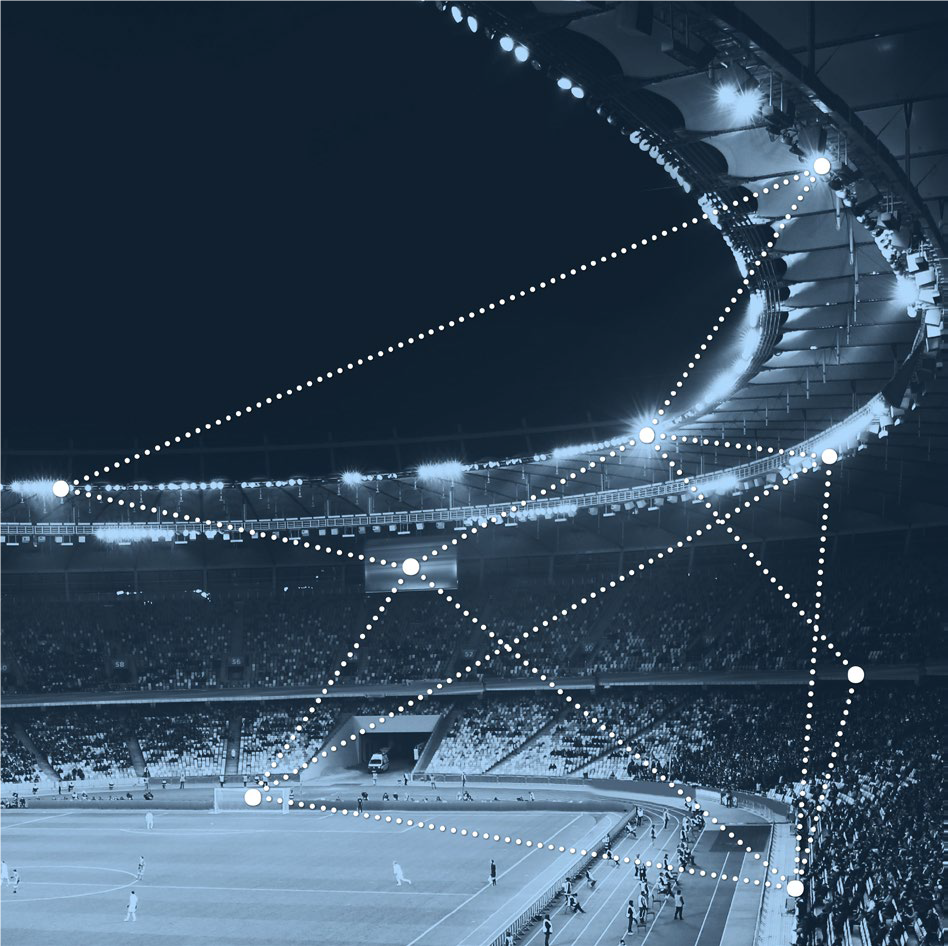
\includegraphics[width=\textwidth]{Bluetooth_Mesh_Stadium_Example.png}
		\caption[Sende-Ablauf mit CCA Busy]{CCA Prüfung (Busy Event) \cite{bluetooth_sig_mesh-technology-overviewpdf_2020}}
		\label{fig:BluetoothMeshStadiumExample}
	\end{minipage}
\end{figure}


Die Technologie baut auf den weit verbreitetem BLE-Standard auf, welcher in einer viel zahl von Endgeräten verbaut ist. Ab BLE-Version 4.2 könnten sich die Geräte zu einem Mesh-Netzwerk verbinden. Bisher wurde der BLE-Standard nur für Point-to-Point Verbindung konzipiert. Das Netzwerk basiert auf dem Managed-Flooding Prinzip. Einfach erklärt wiederholen alle Teilnehmer, bedingt durch verschiedene Abhängigkeiten, jede empfangende Nachricht (Relaying). Somit gelangen die Daten über Zwischenstationen (Hops) zum Ziel. 

\todo[inline]{Bild Managed Flooding}

\todo[inline]{Kurze Einleitung ins Thema Bluetooth Mesh. Dieser Teil ist komplett losgelöst von den anderen Teilen. Es soll klar ersichtlich sein dass dieser Teil durch Raffael Anklin erstellt wurde.}







